\documentclass[dvipdfmx]{beamer}

%%% 以下3つはハンドアウト印刷用
%\documentclass[dvipdfm,handout]{beamer}
%\usepackage{pgfpages}
%\pgfpagesuselayout{4 on 1}[border shrink=3mm]

\AtBeginDvi{\special{pdf:tounicode 90ms-RKSJ-UCS2}}
%\setbeamersize{text margin left=1.5cm}
%\voffset=0.5cm

%%% メインテーマ
%\usetheme{Berkeley}
%\usetheme{CambridgeUS}
%\usetheme{Default}
%\usetheme{Darmstadt}
%\usetheme{Hannover}
%\usetheme{lankton-keynote}
%\usetheme{Luebeck}
%\usetheme{Marburg}
\usetheme{Copenhagen}

%%% カラーテーマ(省略可)
%\usecolortheme{beaver}
%\usecolortheme{beetle}
%\usecolortheme{crane}
%\usecolortheme{dolphin}
%\usecolortheme{seagull}
%\usecolortheme{wolverine}
\useoutertheme{infolines}
\usecolortheme[RGB={51,102,255}]{structure}                                                                                                      
\usecolortheme{seahorse}


\newcommand{\backupbegin}{
\newcounter{framenumberappendix}
\setcounter{framenumberappendix}{\value{framenumber}}
}
\newcommand{\backupend}{
\addtocounter{framenumberappendix}{-\value{framenumber}}
\addtocounter{framenumber}{\value{framenumberappendix}}
}

%%% フォント
\renewcommand{\kanjifamilydefault}{\gtdefault} % 日本語フォントをゴシック
\usefonttheme[onlylarge]{structurebold}
\fontencoding{\encodingdefault}
\fontfamily{\kanjifamilydefault}
\fontseries{\seriesdefault}
\fontshape{\shapedefault}
\selectfont
%\mathversion{bold} % 数式フォントをbold体
\renewcommand{\figurename}{図}
\renewcommand{\tablename}{表}

%%% インナー, アウターテーマ(省略可)
%\useinnertheme{circles}
%\useoutertheme{infolines}


%\logo{\includegraphics[width=1.5cm, height=1.5cm]{.jpg}} % ロゴをいれる
\setbeamertemplate{navigation symbols}{} % ナビゲーションバーなし
%\setbeamertemplate{background}[grid][step=5mm] % 背景グリッド
\setbeamertemplate{footline}[frame number] % ページ番号の表示
\setbeamerfont{footline}{size=\small,series=\bfseries}
\setbeamercolor{footline}{fg=black,bg=black}
\setbeamertemplate{caption}[numbered] % 図表番号の表示
\setbeamerfont*{frametitle}{size=\normalsize,series=\bfseries} % フレーム文字の大きさ

%%% パッケージ
\usepackage[greek,russian,english,french,german,japanese]{babel}
\usepackage{inputenc}
\usepackage{times}
\usepackage{ascmac}
\usepackage{amsmath}
\usepackage{amssymb}
\usepackage{amsfonts}
\usepackage[T1]{fontenc}
\usepackage{hyperref}
\usepackage{mathpazo}
\usepackage{comment}
\usepackage[hang,small,bf]{caption}
\usepackage{color}
\usepackage{algorithm,algorithmic}
\usepackage{listings}
\usepackage{multicol}
\usepackage{colortbl}
%\usepackage{tikz}
%\usetikzlibrary{arrows}
%\tikzstyle{block}=[fill=blue,draw opacity=0.7,line width=1.4cm]

\newcommand{\bm}[1]{\mbox{\boldmath $#1$}}
\newcommand{\mapright}[1]{\mathop{\longrightarrow}\limits_{#1}}
\newcommand{\argmax}{\mathop{\rm argmax}\limits}
\makeatletter
\@float@every@algorithm{\tiny}%%!! 全体をざっくりと \small へ
\makeatother




%%% Title, Author, etc.
\title[タイトル]{粒子フィルタによるデフォルト率分布の推定}
%\subtitle[サブタイトル]{}
\author[発表者名]{塩濱研究室 稗田尚弥}
\institute[所属]{東京理科大学大学院工学研究科経営工学専攻1年 \\ 学籍番号 4417621}
\date[日付]{2017年9月4日}


\begin{document}

\begin{frame}[plain]
\titlepage
\end{frame}


\begin{frame}{目次}
\tableofcontents
\end{frame}

\section{目的・背景}
\begin{frame}{背景}
政府にとって重要な目的の一つは,民間の個人と企業に,安定した経済環境を提供することである.その目的を実現するひとつの方法が,銀行の倒産がほとんどおこらず,信頼のおける銀行システムを提供することである.\\
銀行は,\textcolor{red}{信用創造},金融仲介,決済機能の三つの機能によって,国内外で為替の流通を管理する金融機関である.
それぞれ,\textcolor{red}{融資},預金,決済という形で我々に提供されている.\\
\end{frame}

\begin{frame}
銀行が抱えている次の三つのリスクを適切に把握し,維持すべき資本を算出することは,倒産を回避するために重要な業務である.
\begin{block}{}
\begin{itemize}
 \item \textcolor{red}{信用リスク} 
 \item 市場リスク 
 \item オペレーショナルリスク 
\end{itemize}
\end{block}
本研究ではこのうち,信用リスクにあたる\textcolor{red}{デフォルトリスク}に着目する.
融資によってできるポートフォリオを与信ポートフォリオといい,債務不履行のことを\textcolor{red}{デフォルト}という.
所有している与信ポートフォリオの中の,債務者全体のデフォルト率を把握することは,リスク管理において重要である.
\end{frame}

\begin{frame}{目的}
\begin{itemize}
\item
実際のデフォルト率から,与信ポートフォリオのデフォルト率が従う確率分布を推定する.
\item
デフォルト率の分布は,先行研究より導出される二つの分布を用いて行う.本研究では,時変パラメータを持つVasicek 1-ファクターモデル,Lamb and Perraudin モデルと呼ぶ.
\item
状態の推定方法として,状態空間モデルによるParticleFilterを行い,EMアルゴリズムによってパラメータの推定を行う.
特に,時変パラメータを持つVasicek 1-ファクターモデルは非線形非ガウスなモデルであり,カルマンフィルタで状態を推定することが不可能であるためである.
\end{itemize}
\end{frame}


\section{EMアルゴリズム}

\begin{frame}{状態空間モデル}
状態空間モデルとは,主に時系列解析に使われるモデルで,状態式と観測式から構成される.
本発表においては便宜上,一般の状態変数を$x$,観測変数を$y$で表す.\\
状態空間モデルの一般式は下記のように表される.\\
\begin{center}
状態式:$x_t = P_{\theta}(x_{t-1})$\\
観測式:$y_t = Q_{\theta}(x_{t})\hspace{3.5mm}$
\end{center}
モデルを図で表す.
\begin{figure}[h]
\begin{center}
  \includegraphics[scale=0.41]{figure/state_space.png} \\
\label{fig:state_space}
\end{center}
\caption{状態空間モデル}
\end{figure}
\end{frame}


\begin{frame}{状態空間モデル}
状態空間モデルの主な課題は,既に観測された観測値を用いて,観測できない現在の状態変数と将来の観測値を予測することにある.\\
\begin{itemize}
 \item FIltering:\\
 時点\textcolor{blue}{$1\sim t$}の観測値に基づき,状態変数の時点\textcolor{green}{$t$}の値を推定する.
 \item Smoothing:\\
 時点\textcolor{blue}{$1\sim t$}の観測値に基づき,時点\textcolor{blue}{$1\sim t$}の状態変数の値を推定する.
 \item Prediction:\\
 時点\textcolor{blue}{$1\sim t$}の観測値に基づき,時点\textcolor{red}{$t+1$}の状態変数を推定する.
\end{itemize}
次のスライドよりFilteringとSmoothingの数式とMonte Carlo法による近似について説明する.
\end{frame}

\begin{frame}{Filteringの手順}
Filteringは次のように再帰的に計算ができる.
\begin{enumerate}
 \item 1期前のFiltering分布$F_{t-1}(x_{t-1}|y_{1:t-1})$と,$x_{t-1}$が与えられたもとでの$x_t$の条件付き分布${P_\theta}_{dist}(x_t|x_{t-1})$に基づき,$y_{1:t-1}$が
与えられたもとでの$x_t$の一期先予測分布を求める.
\begin{equation*}
\label{eq:filter1}
{\pi_x}_{t}(x_t|y_{1:t-1})=\int {P_\theta}_{dist}(x_t|x_{t-1})F_{t-1}(x_{t-1}|y_{1:t-1})dx_{t-1}.
\end{equation*} 
 \item 次の観測値の一期先予測分布を求める.
\begin{equation*}
\label{eq:filter2}
{\pi_y}_t(y_t|y_{1:t-1})=\int {Q_\theta}_{dist}(y_t|x_t){\pi_x}_{t}(x_t|y_{1:t-1})dx_t.
\end{equation*}
 \item 事前分布としての$\pi_x(x_t|y_{1:t-1})$と,尤度${Q_\theta}_{dist}(y_t|x_t)$からベイズの定理を適用して,現時点のFiltering分布$F_t(x_t|y_{1:t})$を求める.
\begin{equation*}
F_t(x_t|y_{1:t})=\frac{{Q_\theta}_{dist}(y_t|x_t){\pi_x}_{t}(x_t|y_{1:t-1})}{{\pi_y}_t(y_t|y_{1:t-1})}.
\end{equation*}
\end{enumerate}
\end{frame}

\begin{frame}{Particle Filter}
状態変数の推定密度を求めるには積分計算が必要である.しかし,一般のモデルでは,この計算を解析的に行う事は困難である.\\
よって,Monte Carlo計算によって数値的に行うParticle Filterを用いる.\\
Particle Filterの更新過程は,次の2ステップからなる.\\
状態系列${x}^{(i)}_{0:t-1}$の各点に対し,
\begin{itemize}
\item ${x}^{(i)}_{0:t}$を得るために追加要素$x^{(i)}_t$を$P_\theta$に従ってN個抽出する.\\
\item FilterWeight $\omega_{t-1}^{(i)}$を$\omega_t^{(i)}$に更新する.\\
\end{itemize}
FilterWeightの更新は以下のように表される.
\begin{eqnarray*}
\omega^{(i)}_t\propto
{Q_\theta}_{dist}(y_t|x^{(i)}_t) \cdot  \omega^{(i)}_{t-1}.
\end{eqnarray*}
\end{frame}



\begin{frame}{Particle Filter}
\begin{figure}[h]
\begin{center}
  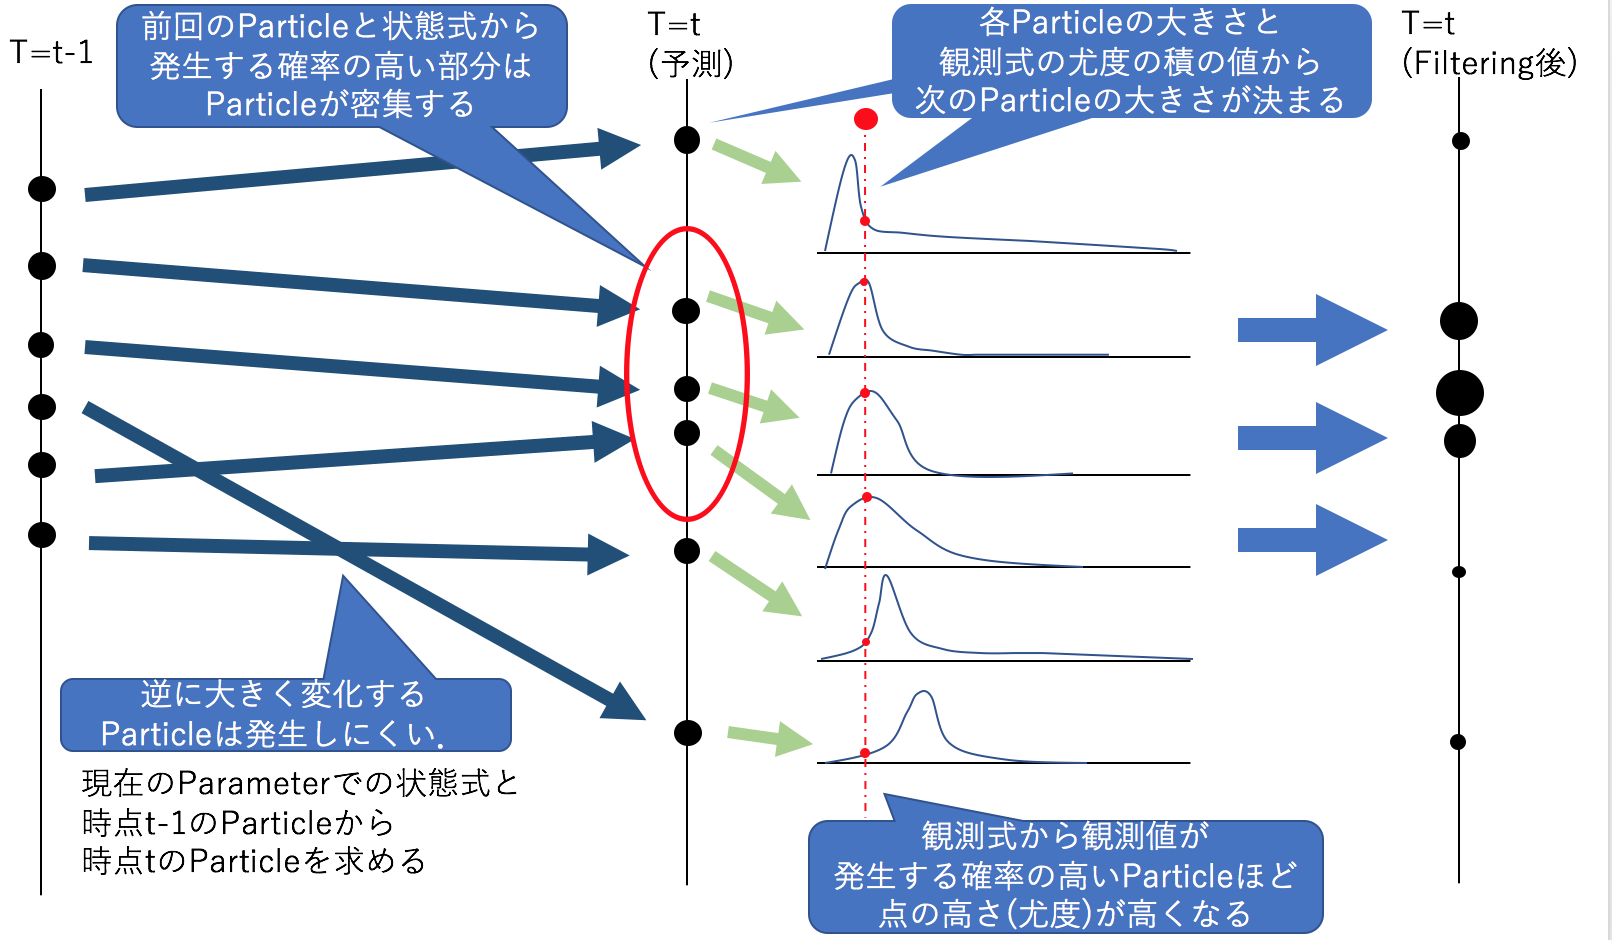
\includegraphics[scale=0.41]{figure/filter_img.png} \\
\label{fig:Em}
\end{center}
\caption{Particle Filter}
\end{figure}
\end{frame}

\begin{frame}{Smoothingの手順}
任意の$t<T$において,$y_{1:T}$が与えられた下での$x_t$のSmoothing分布$S_t(x_t|y_{1:T})$は次のように計算できる.
\begin{enumerate}
 \item $y_{1:T}$の条件付きで,状態の系列$(x_0,\dots x_T)$の後ろ向きの遷移確立を求める.
\begin{equation*}
 S_t(x_t|x_{t+1},y_{1:T})=\frac{{P_\theta}_{dist}(x_{t+1}|x_t){F_x} (x_t|y_{1:t})}{\pi_x(x_{t+1}|y_{1:T})}.
\end{equation*}
 \item $y_{1:T}$が与えられたもとでの$x_t$のSmoothing分布は,次のような$\pi(x_T|y_{1:T})$から始まる$t$の後ろ向き漸化式に従い求めることができる.
\begin{equation*}
S_t(x_t|,y_{1:T})=F(x_t|y_{1:t})\int \frac{P_\theta(x_{t+1}|x_t)}{{\pi_x}_t(x_{t+1}|y_{1:t})}S_{t+1}(x_{t+1}|y_{1:T})dx_{t+1}.
\end{equation*}
\end{enumerate}
\end{frame}

\begin{frame}{Forward Filtering Backward Smoothing}
Smoothingにおいても,積分計算をMonte Carlo計算で行う.Particle Filterによって求めた推定密度から、後ろ向きの遷移確率を求めるためにFFBSを用いる.
Particle FilterのParticle${x}^{(i)}_{0:T}$を用いて,次の計算でSmoothing weigth $\omega_{t|T}^{(i)}$を更新する.
\begin{eqnarray*}
\omega_{t|T}^{(i)}=\omega_{t}^{(i)}\sum_{j=1}^N\omega_{t+1|T}^j\frac{{P_{\theta}}_{dist}(x_t^{(i)}|x_{t+1}^{(j)})}{\sum_{k=1}^{N}\omega_t^{(k)}{P_\theta}_{dist}(x_t^{(k)}|x_{t+1}^{(j)})}
\end{eqnarray*}
\end{frame}


\begin{frame}{Forward Filtering Backward Smoothing}
\begin{figure}[h]
\begin{center}
  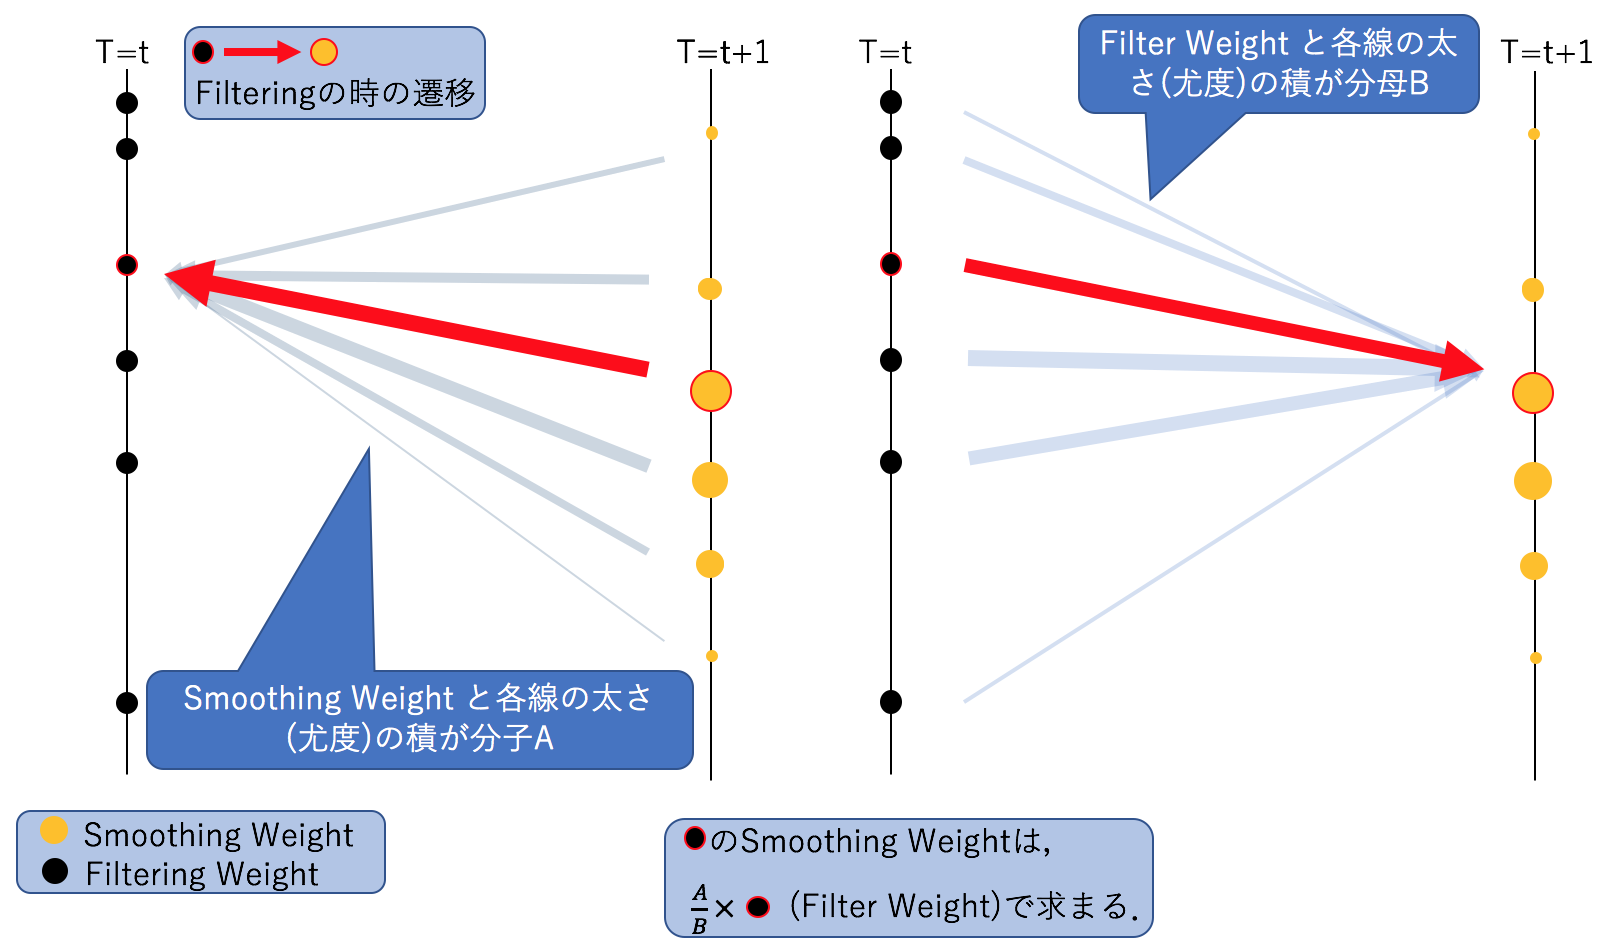
\includegraphics[scale=0.41]{figure/smoothing_img.png} \\
\label{fig:Em}
\end{center}
\caption{Forward Filtering Backward Smoothing}
\end{figure}
\end{frame}




\begin{frame}{EMアルゴリズム}
状態空間モデルに含まれるパラメータを推定するために,状態式と観測式の尤度を最大化したいと考える.
これを効率的に行うために,EMアルゴリズムを用いる.
\begin{itemize}
\item Eステップで,初期パラメータを用いて,FilteringとSmoothingを行い潜在変数の事後分布を求める.
求めた事後分布から、パラメータ集合$\theta$の関数として、対数尤度を求める.
\item Mステップで,パラメータ$\theta$を変化させることで,対数尤度関数が最大になる点を求める.
\end{itemize}
最大化したい尤度関数の対数の期待値EMは以下の式である.
\begin{eqnarray*}
EM(\theta)&=&\int log {P_{\theta0}}_{dist}(x_0)d(x_0)\\
&+&\sum_{t=1}^T \int\int log {P_{\theta}}_{dist}(x_{t-1}|x_{t})d(x_{t-1:t})\\
&+&\sum_{t=0}^T\int log {Q_{\theta}}_{dist}(x_t|y_t) d(x_t)
\end{eqnarray*}
\end{frame}

\begin{frame}{Particle Monte Carlo EM Algorithm}
$EM(\theta)$を,Monte Carlo近似する.具体的には,以下の式になる.
\begin{eqnarray*}
EM(\theta)&=&\sum_{i=1}^N \omega_{0|T}^{(i)} log\hspace{1mm} {P_{\theta0}}_{dist}(X_0^{(i)})\\
&+&\sum_{t=1}^T \sum_{i=1}^N\sum_{j=1}^N \omega_{t|T}^{(ij)} log\hspace{1mm} {P_{\theta}}_{dist}(X_{t-1}^{(i)}|X_{t}^{(j)})\\
&+&\sum_{t=0}^T \sum_{i=1}^N \omega_{t|T}^{(i)} log\hspace{1mm} {Q_{\theta}}_{dist}(X_t^{(i)}|Y_t) 
\end{eqnarray*}
上式の$\omega_{t|T}^{(ij)}$は,Pair Wise Smoothing Weightといい,下記の式で求まる.\\
\begin{eqnarray*}
\omega_{t|T}^{(ij)}=\frac{\omega_{t-1}^i\omega_{t|N}^j {P_\theta}_{dist}(X_{t-1}^{i},X_{t}^{j})}{\sum_{l=1}^N \omega_{t-1}^{l}{P_\theta}_{dost}(X_{t-1}^{l},X_{t}^{j})}
\end{eqnarray*}
\end{frame}


\begin{frame}{Pair Wise Smoothing Weight}
\begin{figure}[h]
\begin{center}
  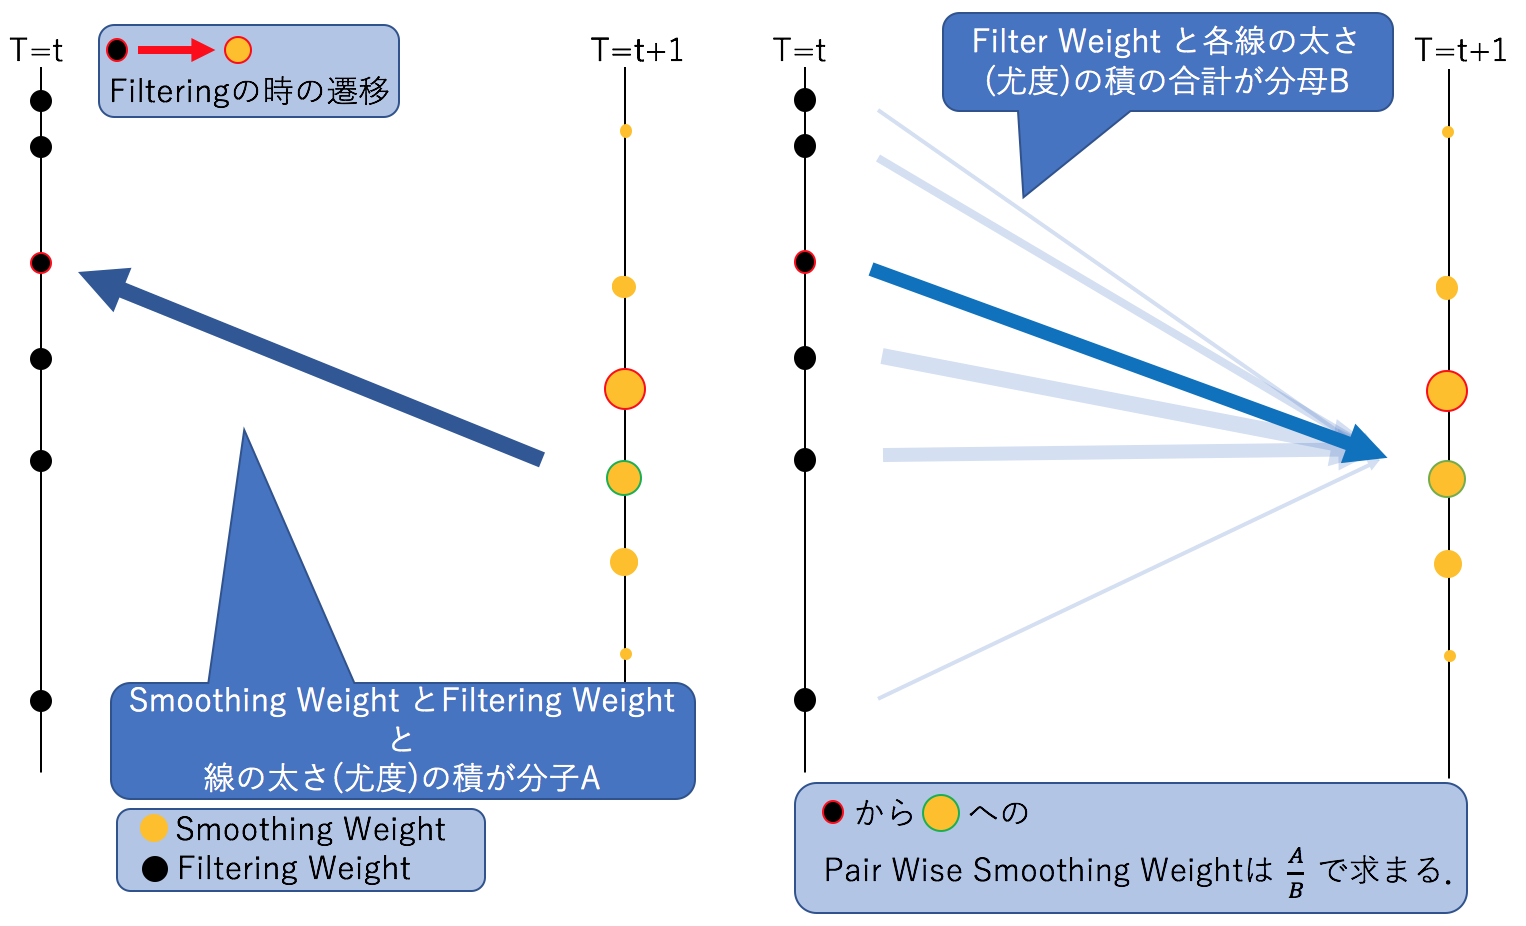
\includegraphics[scale=0.39]{figure/pair_img.png} \\
\label{fig:Em}
\end{center}
\caption{Pair Wise Smoothing Weight}
\end{figure}
\end{frame}

\begin{frame}{MStep}
\begin{figure}[h]
\begin{center}
  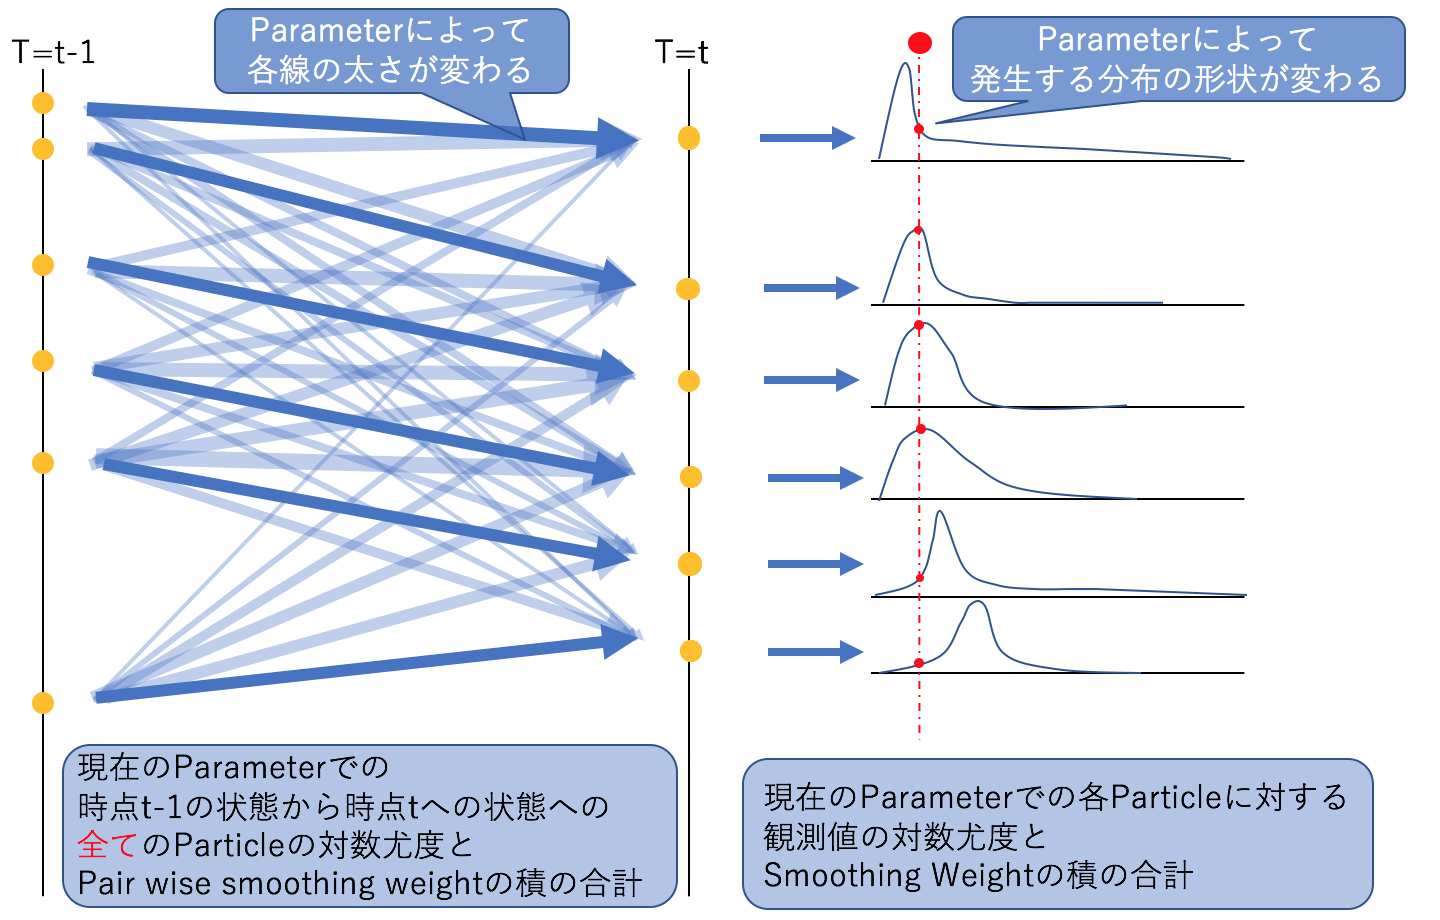
\includegraphics[scale=0.39]{figure/em_img.png} \\
\label{fig:Em}
\end{center}
\caption{Mステップで最大化したい尤度の合計}
\end{figure}
\end{frame}



\section{モデル}
\begin{frame}{時変パラメータを持つVasicek 1-ファクターモデル}
Vasicek and Oldrich によって導出された式より,PDが時変パラメータであると考え,下記のモデルを用いる.
以降,時変パラメータを持つVasicek 1-ファクターモデルとして扱う.\\
状態方程式:
$PD_t=\mu+\phi(PD_{t-1}-\mu)+\varepsilon_t.  \hspace{5mm} \varepsilon_t \sim N(0,sd)$\\
観測方程式:
$
DR_t\sim g(DR_t|PD_t,\rho)
$
\begin{eqnarray}
&&g(DR_t|PD_t,\rho)=\nonumber\\
&&\sqrt{\frac{1- {\rho}}{ {\rho}}} \exp\biggl\{ \frac{1}{2} \biggl[ (N^{-1}(DR))^2 - \biggl( \frac{\sqrt{1- {\rho}}N^{-1}(DR)-N^{-1}({PD_t})}{\sqrt{ {\rho}}}\biggr)^2\biggr]\biggr\}.\nonumber
\end{eqnarray}
\begin{figure}[h]
\begin{center}
  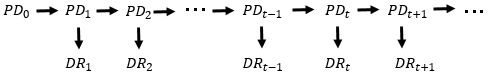
\includegraphics[scale=0.8]{figure/状態空間モデル2.png} \\
\caption{時変パラメータを持つVasicek 1-ファクターモデルの遷移図}
\label{fig:時変パラメータを持つVasicek 1-ファクターモデルの遷移図}
\end{center}
\end{figure}
\end{frame}

\begin{frame}{Lamb and Perraudin モデル}
Lamb and Perraudin の拡張によって導出された下記のモデルを用いる.
状態方程式:$x_t\sim N\left(\sqrt{\beta}x_{t-1} , 1-\beta\right)$\\
観測方程式:$DR_t\sim N\left( \frac{\Phi^{-1}(q)-\sqrt{\rho}\sqrt{\beta}x_{t-1}}{\sqrt{1-\rho}}, \frac{\rho(1 - \beta)}{1 - \rho}\right)$\\ $DR_t$は実際に観測されたデフォルト率を正規分布の逆関数で変換した値\\
$x_t$はマクロエコノミックファクター\\
$\beta$はマクロエコノミックファクターの一次自己相関係数\\
$q$はマートンモデルの閾値\\
$\rho$が、デフォルト率のマクロエコノミックファクターへの感応度
\begin{figure}[h]
\begin{center}
  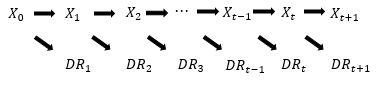
\includegraphics[scale=0.8]{figure/state_space_lamb_and_perraudin.jpg} \\
\caption{Lamb and Perraudin モデルの遷移図}
\label{fig:Lamb and Perraudin モデルの遷移図}
\end{center}
\end{figure}
\end{frame}


\section{データ解析}
\begin{frame}{米国データ}
本研究では,Federal Reserve Board of Banksに
によって発表されている米国の全ての銀行の6つのカテゴリーの損失データを用いる.\\
カテゴリーはそれぞれ,
不動産(RE)・クレジットカード(CC)・その他のローン(OC)・リース(L)・工業(CL)・農業(A)であり,期間は1985年から2016年までの4半期データで128期である.\\
\begin{figure}[h]
\begin{center}
  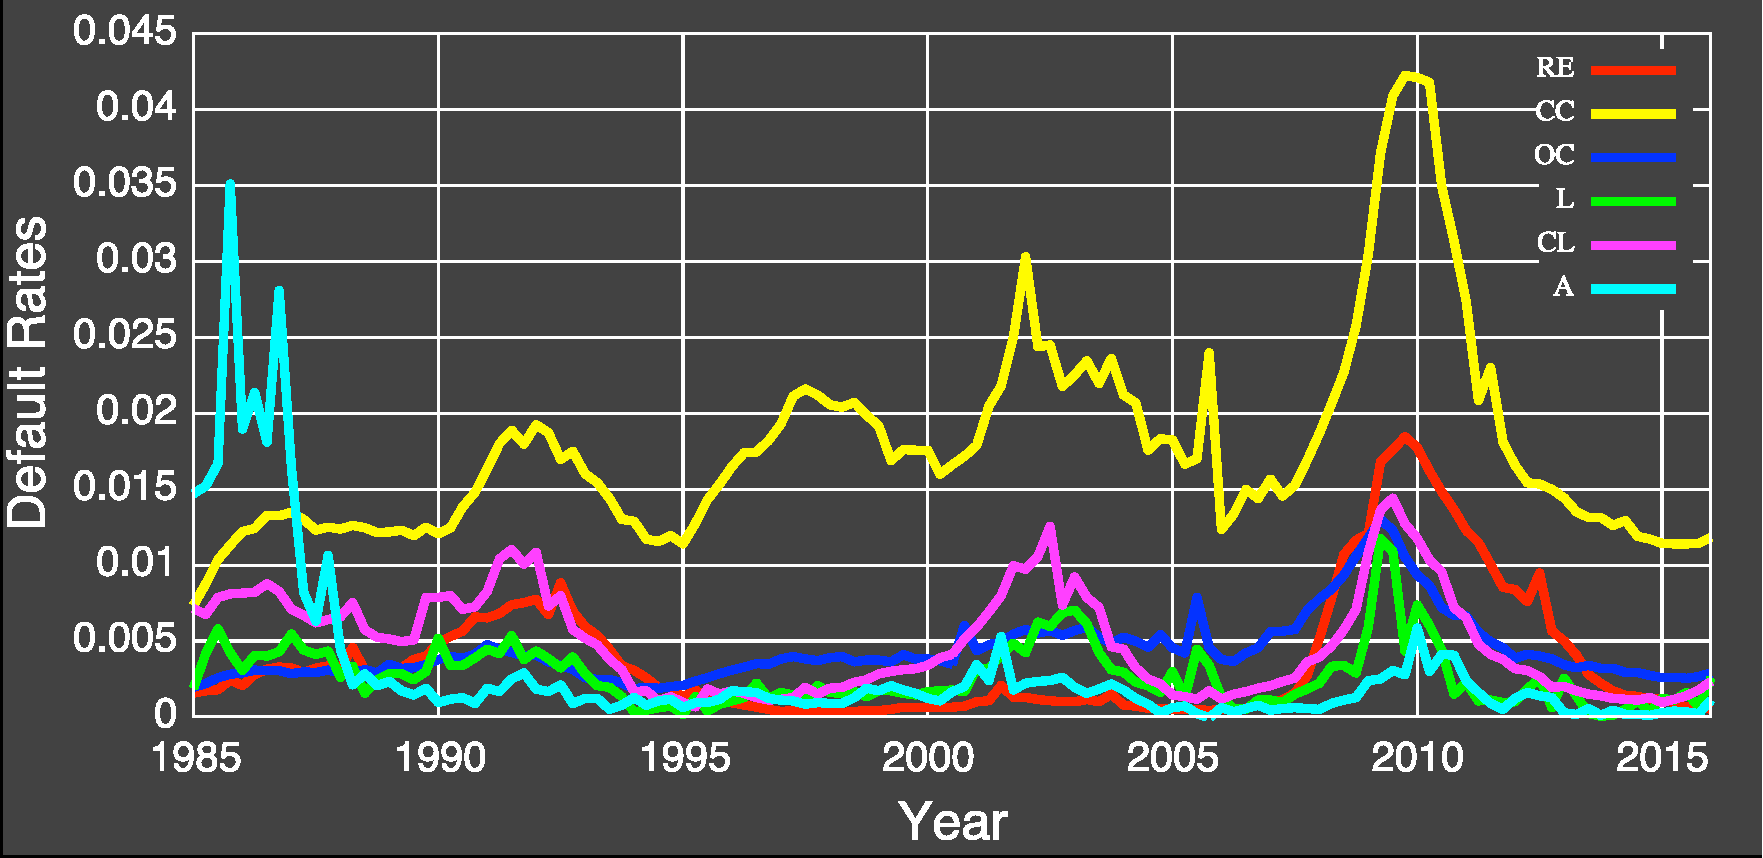
\includegraphics[scale=0.33]{figure/default_data_2016.pdf} \\
\caption{Default Data}
\label{fig:data}
\end{center}
\end{figure}
\end{frame}

\begin{frame}{データ}
データは,四半期ごとに年率変換されたものが,回収額を駆除して発表されているので,四半期あたりの値に変換し,Loss Given Defaultで除算することで,四半期毎のデフォルトデータを算出している.\\
下記は各カテゴリーの基本統計量である.
\begin{table}
\caption{Default Data 基本統計量 (\%)}
\scalebox{0.9}[0.9]{
\begin{tabular}{|l|l|l|l|l|l|l|}\hline
 & RE & CC & OC & L & CL & A \\\hline
mean & 0.370 &\cellcolor[rgb]{1,0.4,0.1} 1.76 & 0.434 &\cellcolor[rgb]{0.1,0.4,1} 0.271 & 0.484 & 0.296 \\\hline
max & 1.85 & \cellcolor[rgb]{1,0.4,0.1}4.22 & 1.30 & \cellcolor[rgb]{0.1,0.4,1}1.18 & 1.44 & 3.51 \\\hline
min & 0.0286 & 0.736 &\cellcolor[rgb]{1,0.4,0.1} 0.185 & 0.00556 & 0.0667 &\cellcolor[rgb]{0.1,0.4,1} 0.000 \\\hline
Volatility & 0.00184 & 0.00456 & 0.000452 &\cellcolor[rgb]{0.1,0.4,1} 0.000404 & 0.00113 &\cellcolor[rgb]{1,0.4,0.1} 0.00286 \\\hline
Acf(1) & \cellcolor[rgb]{1,0.4,0.1}97.3 & 93.6 & 94.0 & \cellcolor[rgb]{0.1,0.4,1}78.3 & 94.4 & 83.6 \\\hline
median & 0.179 &\cellcolor[rgb]{1,0.4,0.1} 1.64 & 0.378 & 0.214 & 0.393 & \cellcolor[rgb]{0.1,0.4,1}0.128 \\\hline
\end{tabular}
}
\end{table}
\end{frame}



\appendix
\backupbegin

\section{先行研究}
\begin{frame}{Limiting Loan Loss Probability Distribution\\Vasicek and Oldrich}
ポートフォリオの損失率を表すモデルとして、Vasicekらによるモデルが提案されている.
ポートフォリオに含まれる各債務者の資産価値$U_i$をOne-factorモデルで定義する.\\
\begin{itemize}
\item
ポートフォリオに含まれる債務者数を$N$件
\item
全ての債務者に共通する変動要因を$F$
\item
債務者$i$の個別の要因を$Z_i$
\item
債務者$i$と債務者$j$の相関係数({資産相関})を\\
Corr($U_i,U_j$)=$\rho$ですべての債務者間で同一であるとする.
\end{itemize}
以上より$U_i$を次のよう定義できる.
\begin{eqnarray*}
\label{eq:eq5}
U_{i}=\sqrt{\rho} F+\sqrt {1-\rho}Z_{i}, \hspace{10pt} F,Z_i\sim i.i.d\hspace{1pt} N(0,1),
\hspace{10pt} i=1,\dots,N.\hspace{10pt}
\vspace{-8pt}
\end{eqnarray*}
債務者$i$の資産$U_i$のデフォルト境界を$U$とすると,
全体の共通要因Fを所与として$U_i$のデフォルト確率は次のようになる.
{\small
\begin{eqnarray*}
\label{eq:eq9}
{\rm Prob}(U_i<U|F)={\rm Prob}\biggl(Z_i<\frac{U-\sqrt{\rho}F}{\sqrt{1-\rho}}\biggr)=
N\biggl(\frac{U-\sqrt{\rho}F}{\sqrt{1-\rho}}\biggr).
\end{eqnarray*}
}
\end{frame}

\begin{frame}{}
債務者$i$がデフォルトする時刻を$T$として,その累積確率分布を$Q$としたときに,$U$が正規分布に従うことから百分位点対応で
\begin{eqnarray*}
N\biggl(\frac{U-\sqrt{\rho}F}{\sqrt{1-\rho}}\biggr)&=&N\biggl(\frac{N^{-1}(Q(T))-\sqrt{\rho}F}{\sqrt{1-\rho}}\biggr). 
\end{eqnarray*}
全ての企業に共通する要因(マクロ経済要因) $F$が与えられたときの条件付き確率である
この確率を,今後「観測されるデフォルト率({$DR$})」とする.
$F\sim N(0,1)$より,$F<N^{-1}(y)$の確率は$y$である.
したがって,
{\small
\begin{equation}
P\biggl(DR>N\biggl(\frac{N^{-1}(PD)-\sqrt{\rho}N^{-1}(y)}{\sqrt{1-\rho}}\biggr)\biggr)=y.\nonumber
\end{equation}
}
\end{frame}
\begin{frame}{}
$G(DR)$を$DR$の周辺分布とすると,
\begin{eqnarray*}
\label{eq:eq14}
&DR = N \biggl(\frac{N^{-1}(PD)+\sqrt{\rho}N^{-1}(G(DR))}{\sqrt{1-\rho}} \biggr)\\ 
\Longleftrightarrow&G(DR) = N \biggl(\frac{\sqrt{1-\rho}N^{-1}(DR)-N^{-1}(PD)}{\sqrt{\rho}} \biggr).
\end{eqnarray*}
したがって,$DR$の確率密度関数は以下の式になる.
\begin{eqnarray*}
\label{eq:eq16}
&g(DR)=\\
&\sqrt{\frac{1- {\rho}}{ {\rho}}} \exp\biggl\{ \frac{1}{2} \biggl[ (N^{-1}(DR))^2 - \biggl( \frac{\sqrt{1- {\rho}}N^{-1}(DR)-N^{-1}({PD})}{\sqrt{ {\rho}}}\biggr)^2\biggr]\biggr\}.
\end{eqnarray*}
実際のデフォルト率DRの従う分布が,パラメータとして持つのは\\
$PD$と$\rho$の二つの値となる.
\end{frame}


\begin{frame}{Dynamic Default Rates \\Lamb and Perraudin }
Lamb and Perraudin は、Vasicek(1991)のモデルを、自己相関を考慮した一般化モデルに拡張している.\\
所有しているポートフォリオに対して,n人の債務者を想定する.t-1時点でデフォルトしていないi番目の債務者が、時点tでデフォルトするかは潜在的な変数$Z_{i,t}$と定数cを用いて、$Z_{i,t}<c$が満たされるときとする.
$Z_{i,t}$は$t=0,1,2,\dots,$と$i=1,2,\dots,n$として、ファクター構造で表す.\\

\begin{equation}
Z_{i,t}=\sqrt{\rho}x_i+\sqrt{1-\rho}\epsilon_{i,t}.\nonumber
\label{eq:factor_1}
\end{equation}
また、$x_t$もファクター構造で表す.
\begin{equation}
x_{t}=\sqrt{\beta}x_{t-1}+\sqrt{1-\beta}\eta_t\nonumber
\label{eq:autocorrelation}
\end{equation}
ここで、$\epsilon_{i,t}$や$\eta_t$は債務者$i,j$間や時点$t$の組み合わせにおいて独立な正規分布に従うとする.
\end{frame}

\begin{frame}
i番目の債務者の無条件なデフォルト確率$q$が、下記を満たすとする.
\begin{eqnarray}
\Phi^{-1}(q)=c.\nonumber
\end{eqnarray}
時点t-1の情報による条件付きデフォルト確率を考える.デフォルトは下記を満たすとき起こる.
\begin{eqnarray}
&&\sqrt{\rho}x_t+\sqrt{1-\rho}\epsilon_{i,t}<c,\nonumber\\
&&\sqrt{\rho}\sqrt{1-\beta}\eta_t+\sqrt{1-\rho}\epsilon_{i,t}<c-\sqrt{\rho}\sqrt{\beta}x_{t-1}.
\label{eq:left}
\end{eqnarray}
\eqref{eq:left}の左辺は$N(0,1-\rho\beta)$に従う.よって、時点t-1までの情報の条件付きデフォルト確率は以下の通りである.
\begin{eqnarray}
q_{i,t}=\Phi(\frac{c-\sqrt{\rho}\sqrt{\beta}x_{t-1}}{\sqrt{1-\rho}\beta}).\nonumber
\end{eqnarray}
\end{frame}

\begin{frame}
共通要因である$\eta_t$と$x_{t-1}$の条件付きデフォルト確率は、債務者間で独立となる.よって、\eqref{eq:left}を$\epsilon$について変形し、$x_{t-1}$の条件付きで$\eta$を積分することで、n人のうちk人がデフォルトする確率P(k,n)を表す.
\begin{eqnarray}
\epsilon_{i,t}&<&
\frac{c-\sqrt{\rho}\sqrt{\beta}x_{t-1}-\sqrt{\rho}\sqrt{1-\beta}\eta_t}
{\sqrt{1-\rho}}\nonumber\\
&&P(k,n)=\nonumber\\
&&
\begin{pmatrix}
n\\
k
\end{pmatrix}
\int_{0}^{1}\Phi(\frac{c-\sqrt{\rho}\sqrt{\beta}x_{t-1}-\sqrt{\rho}\sqrt{1-\beta}\eta_t}{\sqrt{1-\rho}})^k\nonumber\\
&&\times \bigl[
1-
\Phi(
\frac{c-\sqrt{\rho}\sqrt{\beta}x_{t-1}-\sqrt{\rho}\sqrt{1-\beta}\eta_t}{\sqrt{1-\rho}}
)
\bigr]^{n-k}d\Phi(\eta_k)
\label{eq:tt}
\end{eqnarray}
\end{frame}

\begin{frame}
変数変換を行う
\begin{eqnarray}
s(\eta)
&\equiv&
\Phi(
\frac{c-\sqrt{\rho}\sqrt{\beta}x_{t-1}-\sqrt{\rho}\sqrt{1-\beta}\eta_t}{\sqrt{1-\rho}}
)\nonumber\\
W(s)&=&\Phi(
\frac{\sqrt{1-\rho}\Phi^{-1}(s)-c+\sqrt{\rho}\sqrt{\beta}x_{t-1}}{\sqrt{\rho}\sqrt{1-\beta}}
)\nonumber
\end{eqnarray}
また、
\begin{eqnarray}
-d\Phi(f(s))=d\Phi(-f(s))\nonumber
\end{eqnarray}
上記より\eqref{eq:tt}は
\begin{eqnarray}
P(k,n)&=&
-
\begin{pmatrix}
n\\
k
\end{pmatrix}
\int_{0}^{1}s^k(1-s)^{n-k}
\times\nonumber\\
&&d \Phi(
\frac{-(\sqrt{1-\rho}\Phi^{-1}(s)-c+\sqrt{\rho}\sqrt{\beta}x_{t-1})}
{\sqrt{\rho}\sqrt{1-\beta}}
)\nonumber\\
&=&
\begin{pmatrix}
n\\
k
\end{pmatrix}
\int_{0}^{1}s^k(1-s)^{n-k}
\times
dW(s)\nonumber
\end{eqnarray}
\end{frame}

\begin{frame}
債務者数を無限とし、$\theta$をデフォルトする割合(the pool that default)として考える。
\begin{eqnarray}
\lim_{n\rightarrow\infty}\sum_{i=0}^{[n\theta]}P(i,n)
&=&
\int_0^1\bigl(\lim_{n\rightarrow\infty}\sum_{i=0}^{[n\theta]}
\begin{pmatrix}
n\\
i
\end{pmatrix}
s^i(1-s)^{n-i}
\bigr)dW(s)\nonumber\\
&=&
\int_0^11(s<\theta)dW(s)\nonumber\\
&=&
W(\theta)-W(0)=W(\theta)\nonumber
\end{eqnarray}
従って、$x_{t-1}$の条件付きで損失密度は
\begin{eqnarray}
W(\theta_t)\equiv\Phi(\frac{\sqrt{1-\rho}\Phi^{-1}(\theta_t)-\Phi^{-1}(q)+\sqrt{\rho}\sqrt{\beta}x_{t-1}}{\sqrt{\rho}\sqrt{1-\beta}})\nonumber
\end{eqnarray}
よって損失率である$\tilde{\theta}\equiv\Phi^{-1}(\theta_t)$は正規分布に従い、次のように表せる。
\begin{eqnarray}
\tilde{\theta}\equiv\Phi^{-1}(\theta_t)\sim N\bigl(\frac{\Phi^{-1}(q)-\sqrt{\rho}\sqrt{\beta}x_{t-1}}{\sqrt{1-\rho}},
\frac{\rho(1-\beta)}{1-\rho}
\bigr)\nonumber
\end{eqnarray}
\end{frame}



\begin{frame}{予測の手順}
任意の$k>0$において,時点$t$での予測分布は次のように求める.
\begin{enumerate}
 \item 状態の$k$期先予測分布
\begin{equation*}
\pi(x_{t+k}|y_{1:t})=\int\pi(x_{t+k}|x_{t+k-1})\pi(x_{t+k-1}|y_{1:t})dx_{t+k-1}.
\end{equation*}
 \item 観測値の$k$期先予測分布
\begin{equation*}
\pi(y_{t+k}|y_{1:t})=\int \pi(y_{t+k}|x_{t+k})\pi(x_{t+k}|y_{1:t})dx_{t+k}.
\end{equation*}
\end{enumerate}
\end{frame}



\backupend

\end{document}
